\section{Video Tracking Results: Inverse Compositional Affine}


\begin{figure}[H]
  \centering
  % minipage
  \begin{minipage}{.49\textwidth}
    \centering
    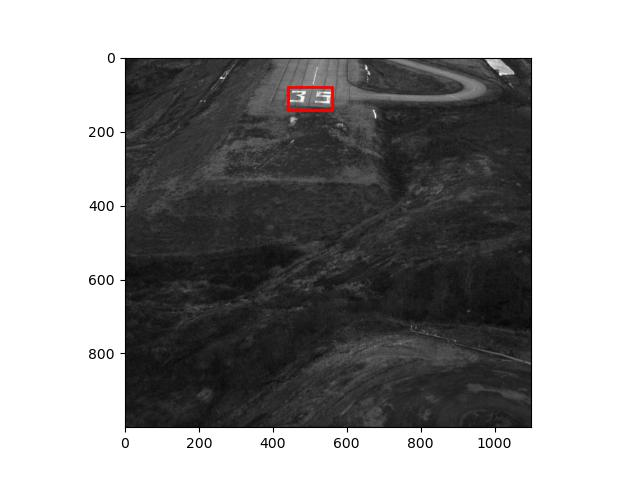
\includegraphics[width=\textwidth]{./figures/ic_affine/landing/frame000001.jpg}
    \caption{Frame $1$}
  \end{minipage}
  \hfill
  % minipage
  \begin{minipage}{.49\textwidth}
    \centering
    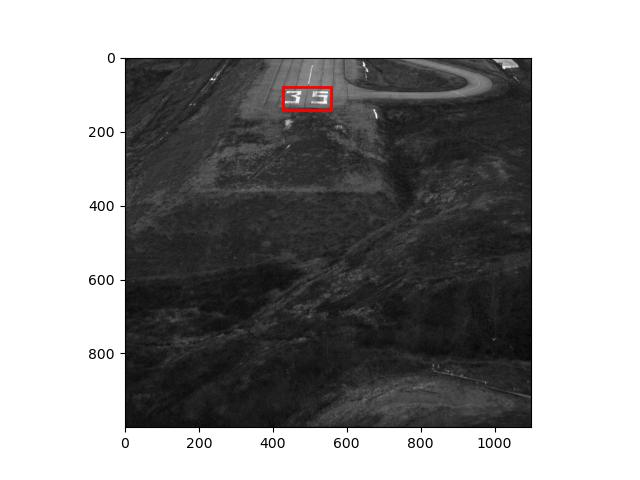
\includegraphics[width=\textwidth]{./figures/ic_affine/landing/frame000010.jpg}
    \caption{Frame $10$}
  \end{minipage}
  \hfill
  % minipage
  \begin{minipage}{.49\textwidth}
    \centering
    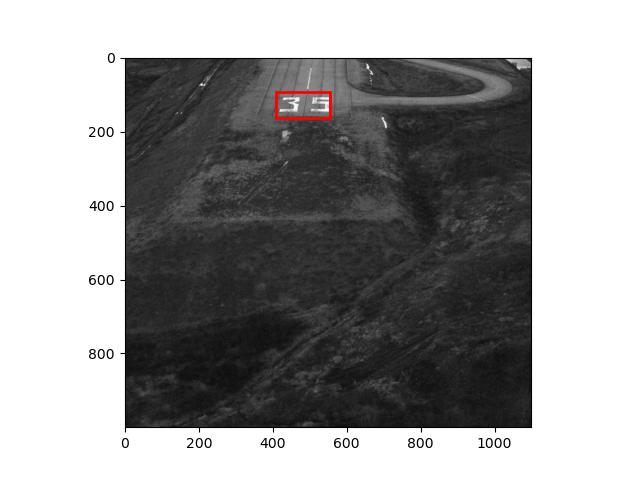
\includegraphics[width=\textwidth]{./figures/ic_affine/landing/frame000020.jpg}
    \caption{Frame $20$}
  \end{minipage}
  % minipage
  \begin{minipage}{.49\textwidth}
    \centering
    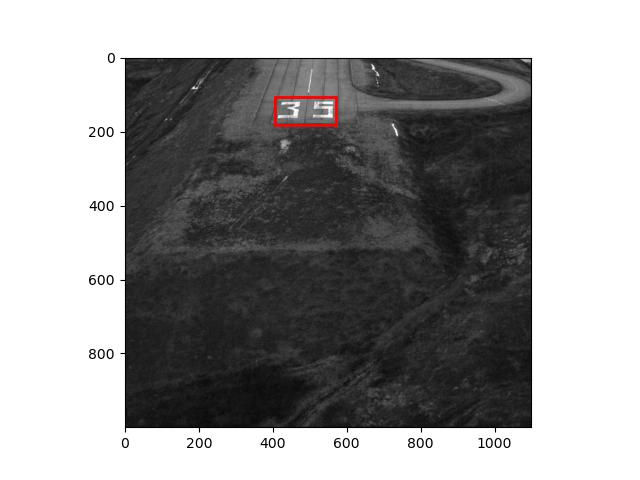
\includegraphics[width=\textwidth]{./figures/ic_affine/landing/frame000030.jpg}
    \caption{Frame $1$}
  \end{minipage}
  \hfill
  % minipage
  \begin{minipage}{.49\textwidth}
    \centering
    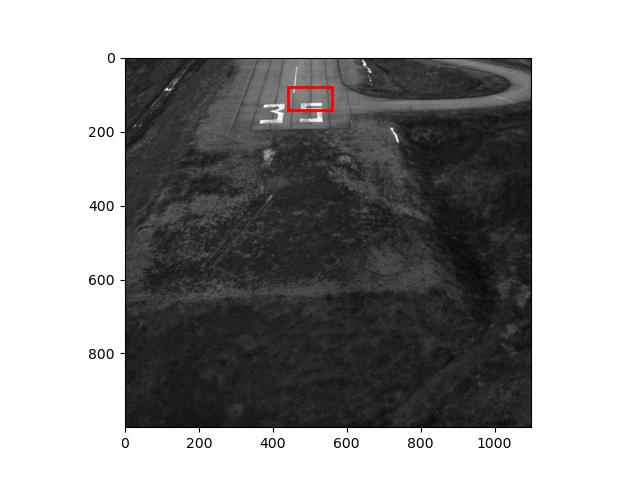
\includegraphics[width=\textwidth]{./figures/ic_affine/landing/frame000040.jpg}
    \caption{Frame $10$}
  \end{minipage}
  \hfill
  % minipage
  \begin{minipage}{.49\textwidth}
    \centering
    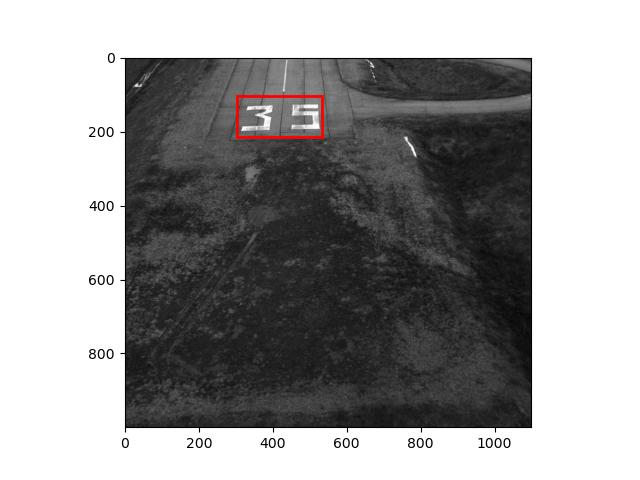
\includegraphics[width=\textwidth]{./figures/ic_affine/landing/frame000049.jpg}
    \caption{Frame $20$}
  \end{minipage}
\end{figure}

%? TWO

\begin{figure}[H]
  \centering
  % minipage
  \begin{minipage}{.49\textwidth}
    \centering
    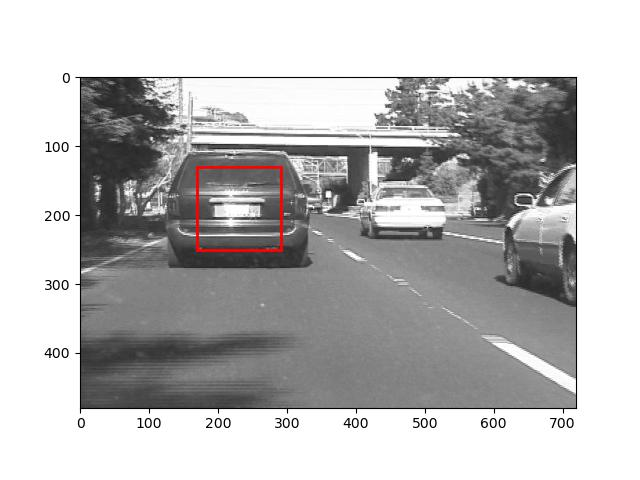
\includegraphics[width=\textwidth]{./figures/ic_affine/car1/frame000001.jpg}
    \caption{Frame $1$}
  \end{minipage}
  \hfill
  % minipage
  \begin{minipage}{.49\textwidth}
    \centering
    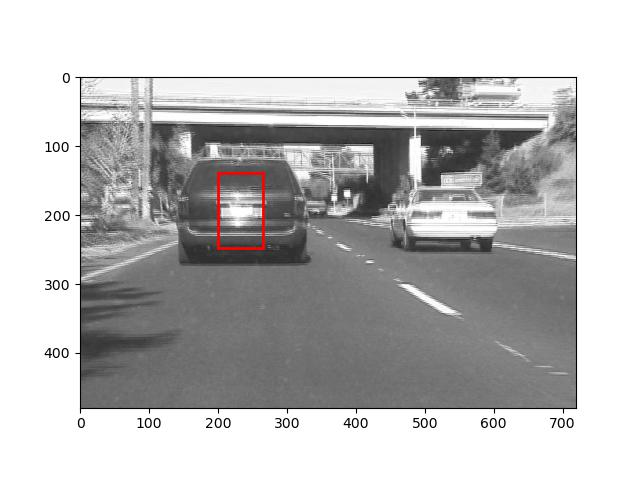
\includegraphics[width=\textwidth]{./figures/ic_affine/car1/frame000050.jpg}
    \caption{Frame $50$}
  \end{minipage}
  \hfill
  % minipage
  \begin{minipage}{.49\textwidth}
    \centering
    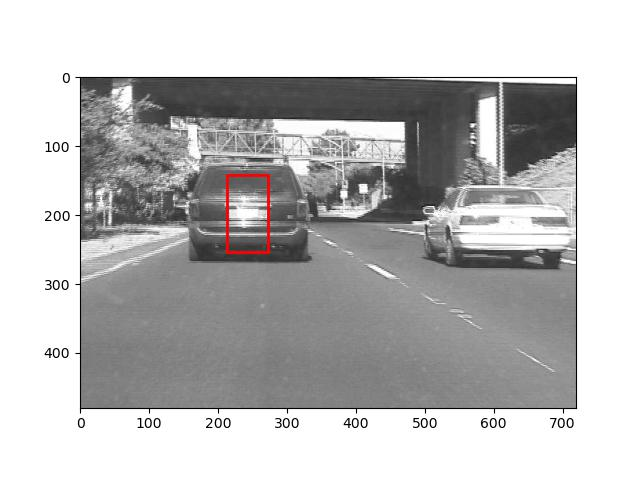
\includegraphics[width=\textwidth]{./figures/ic_affine/car1/frame000100.jpg}
    \caption{Frame $100$}
  \end{minipage}
  % minipage
  \begin{minipage}{.49\textwidth}
    \centering
    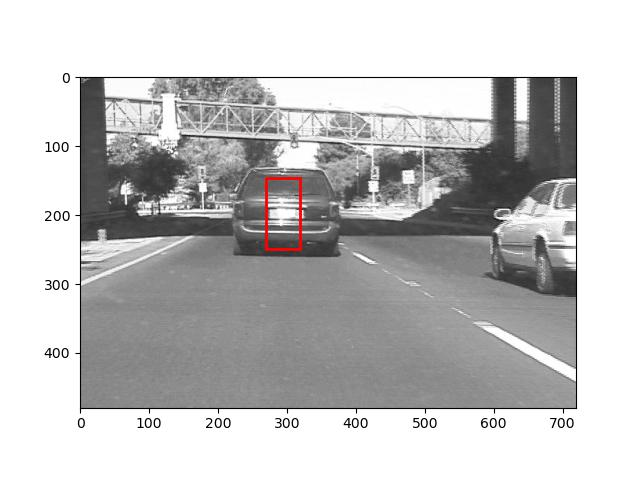
\includegraphics[width=\textwidth]{./figures/ic_affine/car1/frame000150.jpg}
    \caption{Frame $150$}
  \end{minipage}
  \hfill
  % minipage
  \begin{minipage}{.49\textwidth}
    \centering
    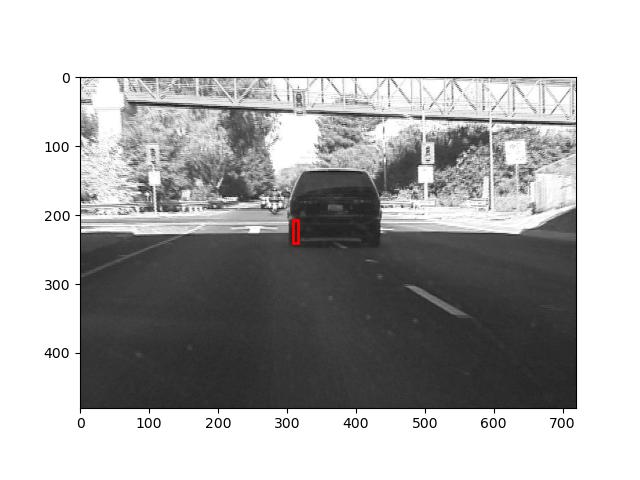
\includegraphics[width=\textwidth]{./figures/ic_affine/car1/frame000200.jpg}
    \caption{Frame $200$}
  \end{minipage}
  \hfill
  % minipage
  \begin{minipage}{.49\textwidth}
    \centering
    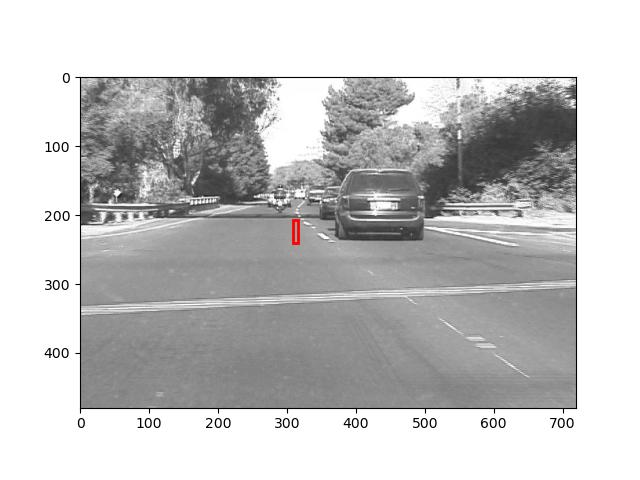
\includegraphics[width=\textwidth]{./figures/ic_affine/car1/frame000250.jpg}
    \caption{Frame $250$}
  \end{minipage}
\end{figure}

%? THREE

\begin{figure}[H]
  \centering
  % minipage
  \begin{minipage}{.49\textwidth}
    \centering
    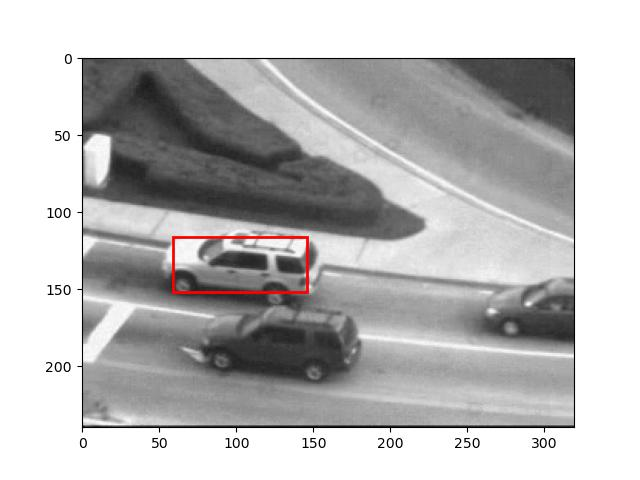
\includegraphics[width=\textwidth]{./figures/ic_affine/car2/frame000001.jpg}
    \caption{Frame $1$}
  \end{minipage}
  \hfill
  % minipage
  \begin{minipage}{.49\textwidth}
    \centering
    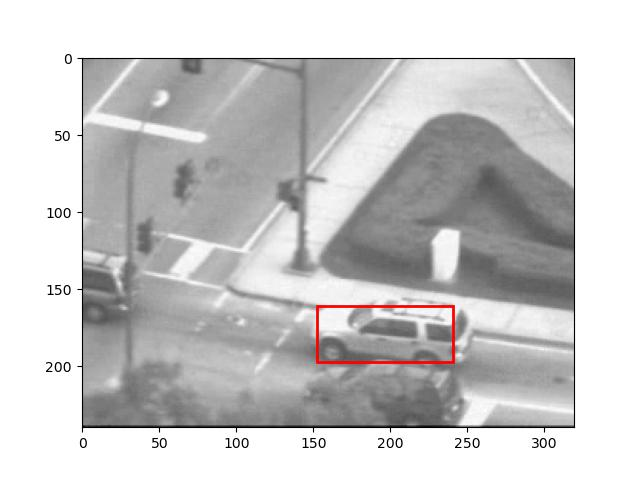
\includegraphics[width=\textwidth]{./figures/ic_affine/car2/frame000050.jpg}
    \caption{Frame $50$}
  \end{minipage}
  \hfill
  % minipage
  \begin{minipage}{.49\textwidth}
    \centering
    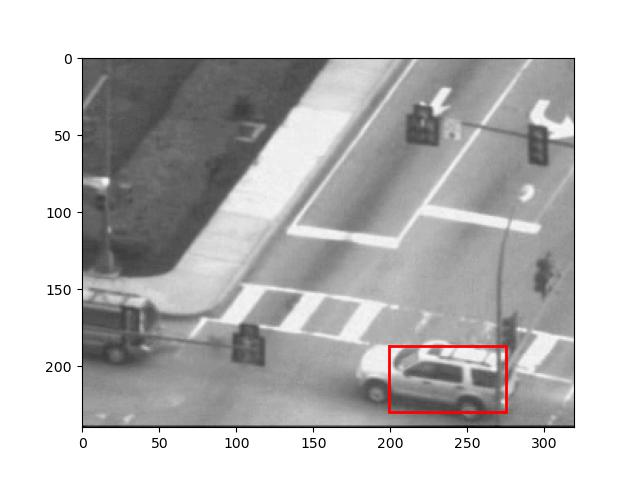
\includegraphics[width=\textwidth]{./figures/ic_affine/car2/frame000100.jpg}
    \caption{Frame $100$}
  \end{minipage}
  % minipage
  \begin{minipage}{.49\textwidth}
    \centering
    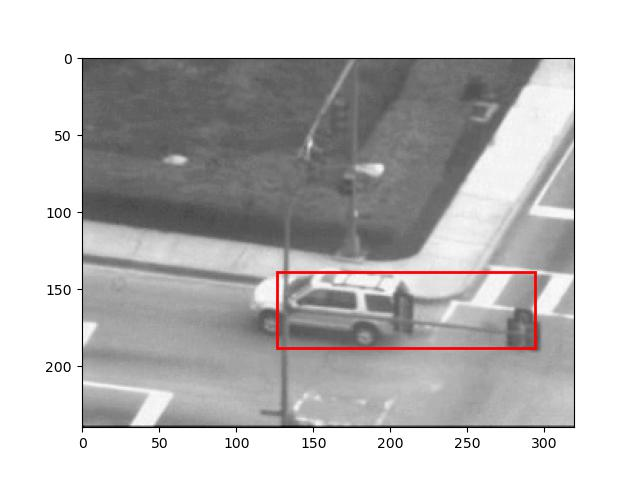
\includegraphics[width=\textwidth]{./figures/ic_affine/car2/frame000150.jpg}
    \caption{Frame $150$}
  \end{minipage}
  \hfill
  % minipage
  \begin{minipage}{.49\textwidth}
    \centering
    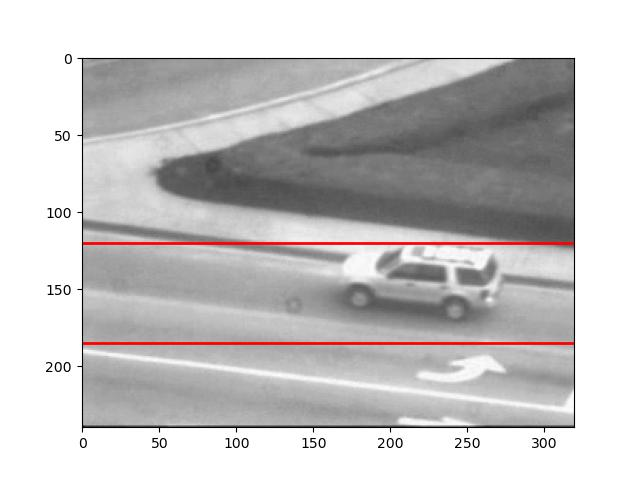
\includegraphics[width=\textwidth]{./figures/ic_affine/car2/frame000200.jpg}
    \caption{Frame $200$}
  \end{minipage}
  \hfill
  % minipage
  \begin{minipage}{.49\textwidth}
    \centering
    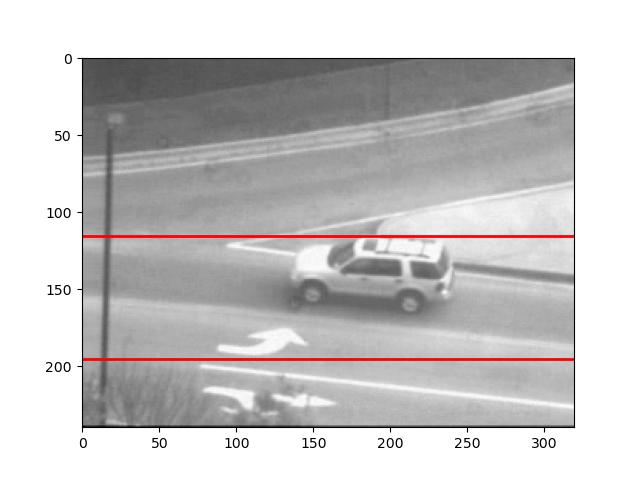
\includegraphics[width=\textwidth]{./figures/ic_affine/car2/frame000250.jpg}
    \caption{Frame $250$}
  \end{minipage}
\end{figure}

\newpage
I noticed that the affine transformations (Lucas-Kanade affine and Inverse-Compositional Affine)
were thrown off in the third video and seemed to stick to one of the street lights
as the car moved.
Here's the exact place where that happens in Inverse-Compositional Affine:

\begin{figure}[H]
  \centering
  % minipage
  \begin{minipage}{.49\textwidth}
    \centering
    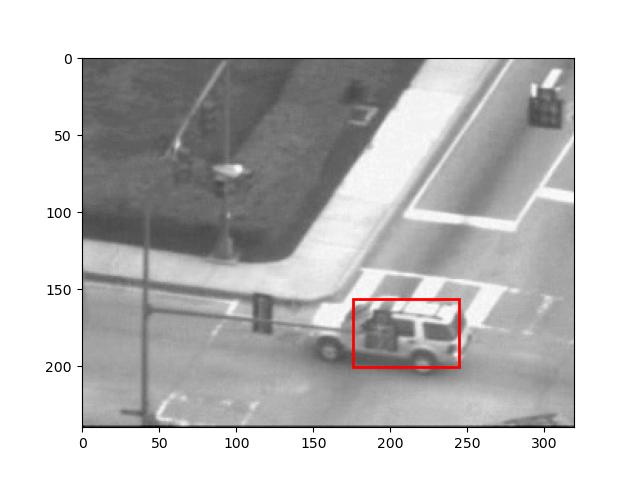
\includegraphics[width=\textwidth]{./figures/ic_affine/car2/frame000125.jpg}
    \caption{Frame $125$}
  \end{minipage}
  \hfill
  % minipage
  \begin{minipage}{.49\textwidth}
    \centering
    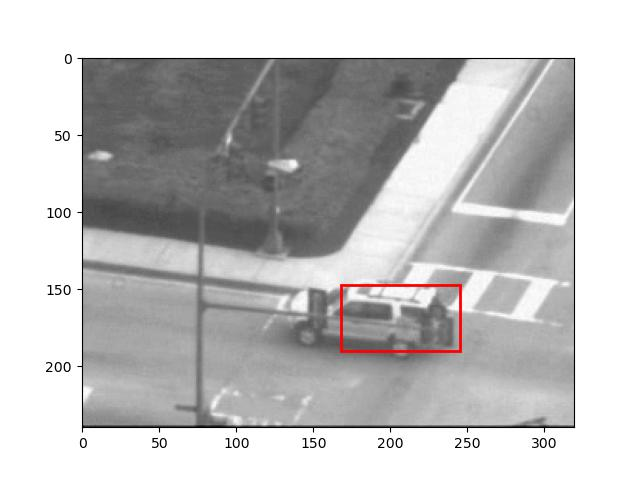
\includegraphics[width=\textwidth]{./figures/ic_affine/car2/frame000135.jpg}
    \caption{Frame $135$}
  \end{minipage}
  \hfill
  % minipage
  \begin{minipage}{.49\textwidth}
    \centering
    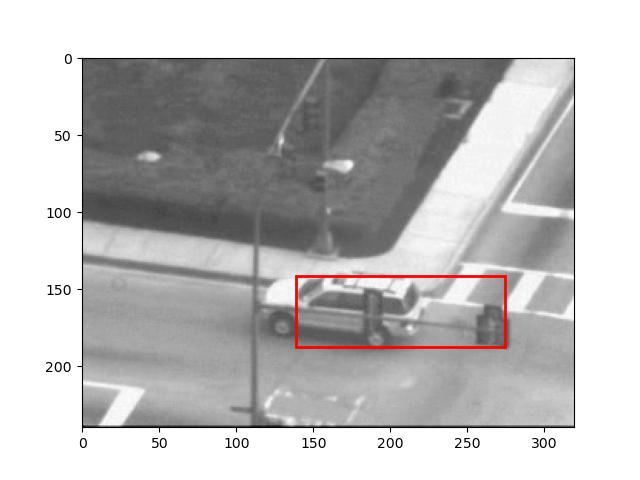
\includegraphics[width=\textwidth]{./figures/ic_affine/car2/frame000145.jpg}
    \caption{Frame $145$}
  \end{minipage}
  % minipage
  \begin{minipage}{.49\textwidth}
    \centering
    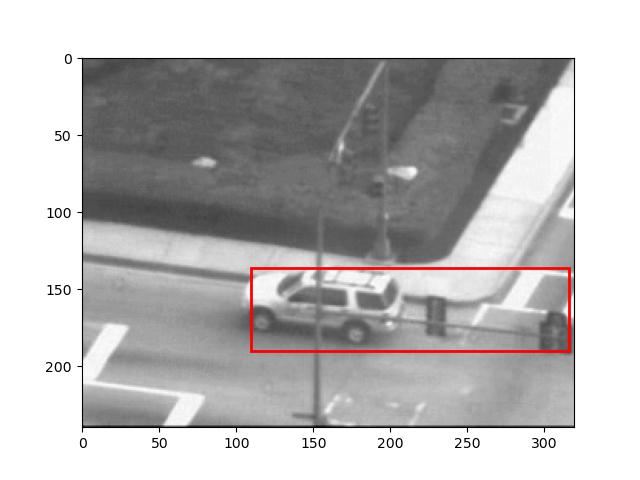
\includegraphics[width=\textwidth]{./figures/ic_affine/car2/frame000155.jpg}
    \caption{Frame $155$}
  \end{minipage}
\end{figure}

Furthermore, I noticed that the bounding box shrinks in \verb|car1| when using
Inverse-Compositional Affine, an issue which does not occur with the other two algorithms.
These errors could be due to an error in the estimation of $\bH^{-1}$
